\subsection{مثال یکپارچه در محدوده دانشگاه}
\label{sec:unified-example}

در یک سناریوی فرضی در محدوده دانشگاه صنعتی امیرکبیر، کاربران وضعیت جای پارک را از میکروسرویس $s$ می‌پرسند. خوشه‌های $C_a$، $C_b$ و $C_c$ به‌ترتیب نماینده همراه اول، ایرانسل و رایتل‌اند. هر خوشه دو دکل دارای سرور لبه دارد و مدیر آن روی سرور شماره ۱ اجرا می‌شود. نام‌ها و داده‌ها برای توضیح روش‌اند و حاصل اندازه‌گیری شبکه واقعی نیستند.

سرورهای خوشه‌ها با $(A_1,A_2)$، $(B_1,B_2)$ و $(C_1,C_2)$ مشخص می‌شوند. هر شش لبه درخواست می‌فرستند، اما $B_2$ نمونه سرویس ندارد و درخواست را با \lr{WRR} به سرور دیگر می‌فرستد. پس مثال شش مبدأ و پنج مقصد دارد.

\begin{figure}[H]
\centering
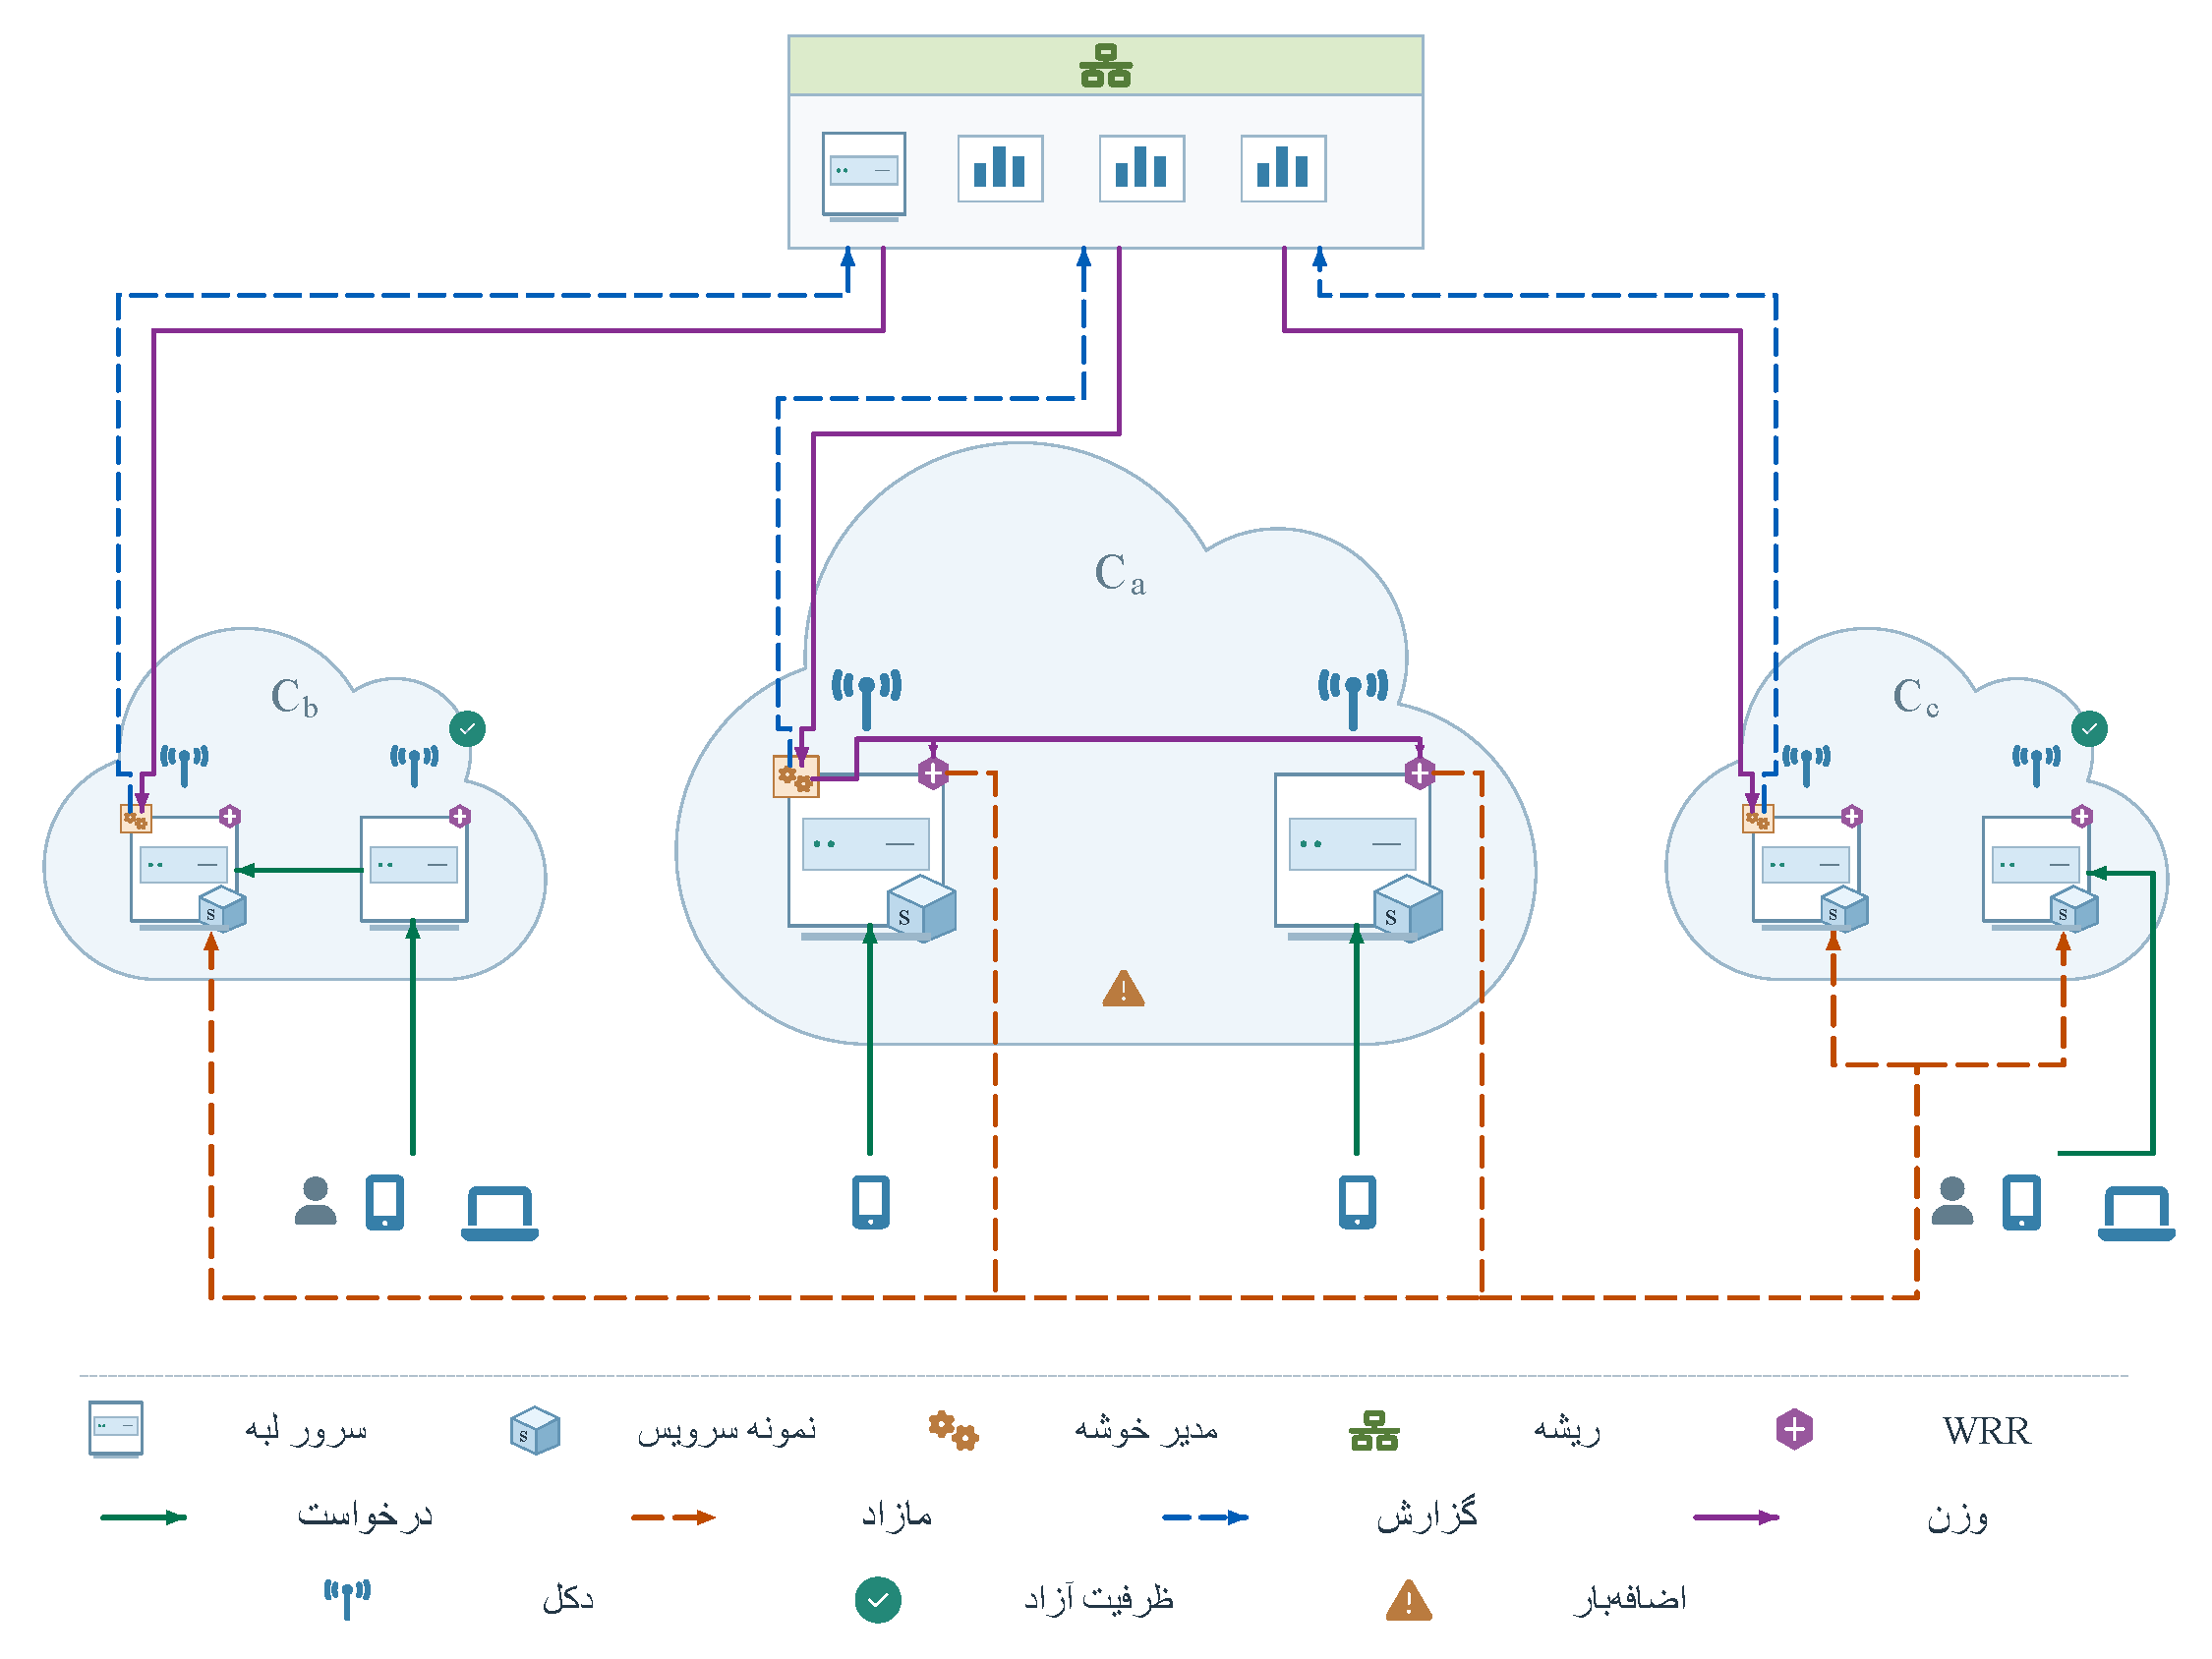
\includegraphics[width=\linewidth]{figures/visio/v10/03-campus-example.pdf}
\caption[مثال سه خوشه با یک لبه بدون سرویس]{سناریوی سه خوشه و شش سرور لبه. هر نماد بدنه، یک سرور است و مکعب، نمونه سرویس را نشان می‌دهد. لبه سمت راست خوشه $C_b$، یعنی $B_2$، مکعب سرویس ندارد و درخواست را به $B_1$ می‌فرستد. ورود کاربران به خوشه‌ها مستقل است. مسیر نارنجی پایین، مجموع ارسال مازاد مبدأهای $C_a$ به مقصدهای خارجی را نشان می‌دهد.}
\label{fig:campus-example}
\end{figure}

\subsubsection{ورودی‌ها و ترتیب محاسبه}

دو جدول زیر داده‌های مسئله را مشخص می‌کنند. پنجره پایش $\Delta=5$ ثانیه، حاشیه اطمینان $\varepsilon=0.1$، ضریب هزینه $\kappa_s=1$ و جریمه شکست $P_s=1$ ثانیه است. در این چرخه، نسبت شکست همه مسیرها و مازاد صف اندازه‌گیری‌شده صفرند؛ پس هزینه ثابت هر مسیر برابر میانگین پینگ همان مسیر است.

\Needspace{12\baselineskip}
\begin{longtable}{>{\centering\arraybackslash}p{1.8cm}>{\centering\arraybackslash}p{2.3cm}>{\centering\arraybackslash}p{1.9cm}>{\centering\arraybackslash}p{3.1cm}>{\centering\arraybackslash}p{3.6cm}}
\caption{استقرار سرویس و داده پردازنده در پنجره قبلی}\label{tab:example-input-hosts}\\
\toprule لبه & نمونه سرویس & هسته $g$ & پردازش پایان‌یافته $N^{\mathrm{proc}}$ & مصرف پردازنده $T^{\mathrm{CPU}}$ \\
\midrule\endfirsthead
\multicolumn{5}{c}{ادامه جدول \ref{tab:example-input-hosts}}\\
\toprule لبه & نمونه سرویس & هسته & پردازش پایان‌یافته & مصرف پردازنده \\
\midrule\endhead\bottomrule\endfoot
$A_1$ & دارد & $2$ & $450$ & $9$ \\
$A_2$ & دارد & $1$ & $270$ & $4.5$ \\
$B_1$ & دارد & $2$ & $285$ & $5.7$ \\
$B_2$ & ندارد & \lr{---} & \lr{---} & \lr{---} \\
$C_1$ & دارد & $2$ & $352$ & $7.04$ \\
$C_2$ & دارد & $1$ & $237$ & $3.95$ \\
\end{longtable}
مصرف پردازنده بر حسب هسته‌ثانیه است و همه ستون‌های پردازشی به کانتینر سرویس $s$ مربوط‌اند. خط تیره در سطر $B_2$ یعنی چنین کانتینری وجود ندارد؛ ظرفیت کل خود سرور صفر فرض نشده است. شمار پردازش‌های پایان‌یافته، همه مبدأهای محلی و خارجی را پوشش می‌دهد و به شمار ارسال یک مبدأ محدود نیست.

\Needspace{12\baselineskip}
\begin{longtable}{>{\centering\arraybackslash}p{1.8cm}>{\centering\arraybackslash}p{3.2cm}>{\centering\arraybackslash}p{3.7cm}>{\centering\arraybackslash}p{3.7cm}}
\caption{تقاضای مبدأها و میانگین پینگ به مقصدهای محلی}\label{tab:example-input-sources}\\
\toprule مبدأ & آغاز تلاش در پنجره $A^{\mathrm{src}}$ & پینگ به مقصد اول & پینگ به مقصد دوم \\
\midrule\endfirsthead
\multicolumn{4}{c}{ادامه جدول \ref{tab:example-input-sources}}\\
\toprule مبدأ & آغاز تلاش & پینگ مقصد اول & پینگ مقصد دوم \\
\midrule\endhead\bottomrule\endfoot
$A_1$ & $612$ & $1$ & $6$ \\
$A_2$ & $408$ & $6$ & $1$ \\
$B_1$ & $180$ & $1$ & \lr{---} \\
$B_2$ & $120$ & $6$ & \lr{---} \\
$C_1$ & $288$ & $1$ & $6$ \\
$C_2$ & $192$ & $6$ & $1$ \\
\end{longtable}
پینگ‌ها بر حسب میلی‌ثانیه‌اند و در هزینه به ثانیه تبدیل می‌شوند. مقصدهای محلی در $C_a$ برابر $(A_1,A_2)$، در $C_b$ فقط $B_1$ و در $C_c$ برابر $(C_1,C_2)$ هستند. برای هم‌میزبانی مبدأ و مقصد، مقدار $1$ میلی‌ثانیه نماینده مسیر محلی فراخوانی سرویس است. اتصال و مجوز دسترسی به همه مقصدهای نشان‌داده‌شده فراهم فرض می‌شود.

مدیر هر خوشه ابتدا سطر مبدأ شماره ۱ و سپس سطر شماره ۲ را حل می‌کند. نرخ‌های تقاضا از تقسیم شمار آغاز تلاش بر $5$ به دست می‌آیند:
\begin{equation}
 \boldsymbol D=(122.4,81.6,36,24,57.6,38.4),\qquad
 (D_{as},D_{bs},D_{cs})=(204,60,96).
\end{equation}
شمار آغاز تلاش و شمار پردازش پایان‌یافته دو شمارنده متفاوت‌اند. درخواست‌های در حال اجرا در مرز پنجره و جابه‌جایی میان خوشه‌ها سبب می‌شوند این دو شمار در یک سطر یا یک پنجره لزوما برابر نباشند.

\subsubsection{برآورد ظرفیت و تعیین سهم محلی}

برای نمونه $A_2$، روابط برآورد خطی چنین نتیجه می‌دهند:
\begin{equation}
 u_{sA_2}=\frac{4.5}{1\times5}=0.9,\qquad
 y_{sA_2}=\frac{270}{5}=54,\qquad
 \mu_{sA_2}=\frac{54}{0.9}=60.
\end{equation}
به همین ترتیب، با ترتیب مقصدهای $(A_1,A_2,B_1,C_1,C_2)$ داریم
\begin{align}
 \boldsymbol u&=(0.9,0.9,0.57,0.704,0.79),\\
 \boldsymbol\mu&=(100,60,100,100,60),\\
 \boldsymbol U&=(1-\varepsilon)\boldsymbol\mu=(90,54,90,90,54),\\
 (K_{as},K_{bs},K_{cs})&=(144,90,144).
\end{align}
واحد ظرفیت و نرخ، درخواست بر ثانیه است. چون $B_2$ نمونه سرویس ندارد، در جمع ظرفیت خوشه $C_b$ وارد نمی‌شود. با مقایسه تقاضا و ظرفیت محلی، نتیجه زیر به دست می‌آید:
\begin{align}
 (\eta_{as},\eta_{bs},\eta_{cs})&=(12/17,1,1),\\
 \boldsymbol\ell&=(86.4,57.6,36,24,57.6,38.4),\\
 \boldsymbol z&=(36,24,0,0,0,0).
\end{align}
پس فقط مبدأهای $C_a$ مازاد دارند و مجموع نرخ خارجی برابر $60$ است. خوشه‌های $C_b$ و $C_c$ ابتدا تقاضای مبدأهای خود را رزرو می‌کنند و سپس ظرفیت باقی‌مانده را به ریشه گزارش می‌دهند.

\subsubsection{حل مدیرهای خوشه}

در این مثال $\kappa_s=1$ است. برای کوتاه شدن نوشتن دستگاه‌ها، مشتق هزینه یک مقصد با ظرفیت $\mu$ و هزینه ثابت $d$ را چنین می‌نویسیم:
\begin{equation}
 G_{\mu,d}(r)=\frac{r(2\mu-r)}{(\mu-r)^2}+2dr.
\end{equation}
در جواب داخلی، مشتق مقصدها برابر $\nu$ و در مقصد روی سقف، $G_{\mu,d}(r)\leq\nu$ است. تخصیص سطرهای قبلی از سقف باقی‌مانده کم می‌شود، اما $\mu$ ثابت می‌ماند.

\paragraph{خوشه همراه اول.}
برای مبدأ $A_1$، سقف‌ها $(90,54)$ هستند و دستگاه به صورت زیر است:
\begin{equation}
\left\{\begin{aligned}
 \frac{r_1(200-r_1)}{(100-r_1)^2}+0.002r_1&=\nu,\\
 \frac{r_2(120-r_2)}{(60-r_2)^2}+0.012r_2&=\nu,\\
 r_1+r_2&=86.4.
\end{aligned}\right.
\end{equation}
با جایگذاری $r_2=86.4-r_1$ و حل در بازه مجاز، جواب و وزن شرطی محلی عبارت‌اند از
\begin{align}
 \boldsymbol r_{A_1}&\simeq(54.504863,31.895137),\qquad \nu\simeq3.940377,\\
 \boldsymbol w_{A_1}&=\boldsymbol r_{A_1}/86.4\simeq(0.630843,0.369157).
\end{align}
هر دو نرخ زیر سقف‌اند. برای مبدأ $A_2$، سقف باقی‌مانده $(35.495137,22.104863)$ است و مجموع آن دقیقا به نرخ محلی $57.6$ می‌رسد. بنابراین، جواب این سطر مستقیما از قید مجموع و سقف‌ها مشخص می‌شود:
\begin{align}
 \boldsymbol r_{A_2}&\simeq(35.495137,22.104863),\\
 \boldsymbol w_{A_2}&\simeq(0.616235,0.383765).
\end{align}
در این سطر، هزینه‌های ثابت به‌ترتیب $0.006$ و $0.001$ هستند. مشتق‌ها روی دو سقف تقریبا $1.829281$ و $1.551101$ می‌شوند؛ انتخاب $\nu=2$ هر دو نامساوی سقف را برقرار می‌کند. مجموع تخصیص محلی $C_a$ برابر $(90,54)$ است و ظرفیت عادی آزاد ندارد.

\paragraph{خوشه ایرانسل و لبه بدون سرویس.}
تنها مقصد محلی سرویس در این خوشه $B_1$ است. برای مبدأ $B_1$، قید مجموع نرخ را برابر $36$ و برای مبدأ $B_2$ آن را برابر $24$ قرار می‌دهد. نرخ دوم از سقف باقی‌مانده $90-36=54$ کمتر است؛ در نتیجه
\begin{equation}
 r_{B_1\rightarrow B_1}=36,\qquad
 r_{B_2\rightarrow B_1}=24,\qquad
 w_{B_1\rightarrow B_1}=w_{B_2\rightarrow B_1}=1.
\end{equation}
برای این دو سطر، مقدارهای $\nu$ به‌ترتیب $G_{100,0.001}(36)=1.513406$ و $G_{100,0.006}(24)\simeq1.019302$ هستند. هر دو جواب داخلی و مجازند. لبه $B_2$ فقط وزن ارسال را به کار می‌برد؛ مجموع نرخ پردازش محلی روی کانتینر $B_1$ برابر $60$ است.

\paragraph{خوشه رایتل.}
برای مبدأ $C_1$، دستگاه با سقف $(90,54)$ عبارت است از
\begin{equation}
 G_{100,0.001}(r_1)=G_{60,0.006}(r_2)=\nu,\qquad r_1+r_2=57.6.
\end{equation}
حل آن، $\boldsymbol r_{C_1}\simeq(36.871360,20.728640)$ و $\nu\simeq1.583011$ است. پس سقف سطر بعد $(53.128640,33.271360)$ می‌شود. برای مبدأ $C_2$ داریم
\begin{equation}
 G_{100,0.006}(r_1)=G_{60,0.001}(r_2)=\nu,\qquad r_1+r_2=38.4.
\end{equation}
جواب این سطر $\boldsymbol r_{C_2}\simeq(22.132591,16.267409)$ و $\nu\simeq0.914849$ است. هر دو سطر زیر سقف‌های مربوط به خود قرار دارند. وزن‌ها و مجموع تخصیص محلی این خوشه عبارت‌اند از
\begin{align}
 \boldsymbol w_{C_1}&\simeq(0.640128,0.359872),\\
 \boldsymbol w_{C_2}&\simeq(0.576370,0.423630),\\
 \boldsymbol R^{\mathrm{plan}}_c&\simeq(59.003950,36.996050).
\end{align}

\subsubsection{حل ریشه و ترکیب وزن‌ها}

هر مدیر، ظرفیت خالی همان کانتینرها را پس از رزرو محلی محاسبه می‌کند. با ترتیب پنج مقصد اعلام‌شده داریم
\begin{equation}
 \boldsymbol S=\boldsymbol U-\boldsymbol R^{\mathrm{plan}}
 \simeq(0,0,30,30.996050,17.003950).
\end{equation}
در نتیجه $A_{as}=0$، $A_{bs}=30$ و $A_{cs}=48$ است. مجموعه پذیرنده‌ها $\mathcal R_s=\{b,c\}$، مجموع ظرفیت آزاد $V_s=78$ و نرخ مازاد $O_s=60$ می‌شود. چون $O_s<V_s$، ریشه از شاخه عادی استفاده می‌کند:
\begin{equation}
 (\pi_{sa},\pi_{sb},\pi_{sc})=(0,5/13,8/13).
\end{equation}
خوشه $C_b$ یک نمونه دارد، پس $v_{sb1}=1$ است. سهم دو نمونه خوشه $C_c$ از تقسیم ظرفیت خالی هر کدام بر $48$ به دست می‌آید:
\begin{equation}
 (v_{sc1},v_{sc2})\simeq(0.645751,0.354249).
\end{equation}
نرخ کل خارجی به $C_b$ برابر $60(5/13)=23.076923$ و به $C_c$ برابر $60(8/13)=36.923077$ است. ریشه همین سهم‌ها را به مدیر مبدأ می‌دهد.

مدیر $C_a$، وزن محلی هر مبدأ را در $12/17$ و سهم خارجی آن را در $5/17$ ضرب می‌کند. برای نمونه، دو درایه خروجی مبدأ $A_1$ چنین محاسبه می‌شوند:
\begin{align}
 W_{A_1,s,a,1}&\simeq(12/17)(0.630843)=0.445301,\\
 W_{A_1,s,b,1}&=(5/17)(5/13)(1)\simeq0.113122.
\end{align}
برای هر مقصد خارجی، حاصل‌ضرب سهم خوشه و نمونه برابر $S_i/78$ است. بنابراین وزن خارجی هر مبدأ $C_a$ برابر $(5/17)S_i/78$ می‌شود. مبدأهای $C_b$ و $C_c$ مازاد ندارند و وزن‌هایشان فقط از حل محلی می‌آید.

\paragraph{کنترل مجموع و ظرفیت.}
وزن‌های هر سطر نامنفی‌اند و مجموع آن‌ها یک است. برای سطرهای $C_a$، مجموع وزن محلی $12/17$ و مجموع وزن خارجی $5/17$ است. نرخ مقصد از جمع سهم همه مبدأها به دست می‌آید، نه فقط از یک مبدأ:
\begin{equation}
 L_i=\sum_e D_{es}W_{esi}.
\end{equation}
با ترتیب $(A_1,A_2,B_1,C_1,C_2)$، نرخ‌های کل حاصل عبارت‌اند از
\begin{equation}
 \boldsymbol L\simeq(90,54,83.076923,82.847065,50.076011)
 \ \leq\ (90,54,90,90,54).
\end{equation}
مجموع نرخ‌ها $360$ و برابر مجموع تقاضای شش مبدأ است. نرخ خارجی هر مقصد $(60/78)S_i$ است و از ظرفیت آزاد آن کمتر می‌ماند. این بررسی برای داده ثابت همین چرخه است.

\subsubsection{حالت‌های دیگر همین استقرار}

در حالت‌های زیر، استقرار پنج نمونه ثابت می‌ماند و فقط ورودی چرخه تغییر می‌کند. سقف خوشه‌ها همچنان $(144,90,144)$ است، مگر آنکه خرابی مقصد ذکر شود.
\begin{enumerate}[label=\arabic*.,leftmargin=*]
\item \textbf{ظرفیت محلی کافی یا برابری با سقف.}
با تقاضای $(100,60,96)$، همه درخواست‌ها محلی‌اند و وزن‌های دو مبدأ $C_a$ به‌ترتیب $(0.639152,0.360848)$ و $(0.578102,0.421898)$ می‌شوند. با تقاضای $C_a$ برابر $144$ نیز سهم محلی یک است و مسیر خارجی فعال نمی‌شود.
\item \textbf{کمبود ظرفیت کل.}
با تقاضای $(330,75,120)$، مازاد $C_a$ برابر $186$ و ظرفیت آزاد پذیرنده‌ها $(15,24)$ است. اضافه بر ظرفیت، یعنی $147$، به دو سهم $73.5$ تقسیم می‌شود؛ در نتیجه نرخ خارجی $C_b$ برابر $88.5$ و نرخ خارجی $C_c$ برابر $97.5$ است. نرخ نهایی تنها میزبان $C_b$ به $163.5$ و دو میزبان $C_c$ به $(126.75,90.75)$ می‌رسد. این توزیع موقت، ظرفیت پردازشی تازه ایجاد نمی‌کند و به افزایش ظرفیت نیاز دارد.
\item \textbf{نبود پذیرنده خارجی.}
با تقاضای $(200,100,170)$، هر سه خوشه مازاد دارند. مازاد $C_a$ برابر $56$ است و موقتا به دو سهم $28$ میان میزبان‌های همان سرویس تقسیم می‌شود؛ بار آن‌ها $(118,82)$ خواهد شد. لبه بدون سرویس $B_2$ حتی در این شاخه مقصد پردازش نیست.
\item \textbf{خرابی یا نبود تقاضا.}
با خرابی $A_2$ و تقاضای $(100,60,96)$، ظرفیت $C_a$ به $90$ می‌رسد؛ وزن مقصد خراب صفر و نرخ خارجی $10$ می‌شود. اگر تقاضای $C_a$ صفر باشد، مبدأهای آن ارسالی ندارند و وزنی از تقسیم بر نرخ صفر ساخته نمی‌شود.
\item \textbf{افزایش خطای مسیر.}
در حالت تقاضای محلی $C_a$ برابر $100$، افزایش نسبت شکست مسیر $A_1$ به $A_1$ از صفر به $0.1$، هزینه ثابت آن را از $0.001$ به $0.101$ ثانیه می‌رساند. با ثابت ماندن سایر ورودی‌های همان سطر، وزن این مقصد از $0.639152$ به $0.402205$ کاهش می‌یابد.
\end{enumerate}

\Needspace{20\baselineskip}
\subsubsection{ماتریس نهایی وزن‌ها}

ماتریس زیر خروجی داده‌های دو جدول ورودی است. هر سطر یک مبدأ و هر ستون یک مقصد دارای سرویس را نشان می‌دهد. نرخ ارسال به هر مقصد، حاصل‌ضرب وزن در تقاضای همان سطر است.

\begin{equation}
\mathbf W_s\simeq
\bordermatrix{
 & A_1 & A_2 & B_1 & C_1 & C_2\cr
A_1 & 0.445301 & 0.260581 & 0.113122 & 0.116878 & 0.064117\cr
A_2 & 0.434989 & 0.270893 & 0.113122 & 0.116878 & 0.064117\cr
B_1 & 0 & 0 & 1 & 0 & 0\cr
B_2 & 0 & 0 & 1 & 0 & 0\cr
C_1 & 0 & 0 & 0 & 0.640128 & 0.359872\cr
C_2 & 0 & 0 & 0 & 0.576370 & 0.423630\cr
}.
\label{eq:example-weight-matrix}
\end{equation}
لبه $B_2$ فرستنده است و سطر دارد، اما چون سرویس ندارد، ستون ندارد. دو سطر خوشه $C_b$ به علت وجود تنها یک مقصد محلی برابرند؛ وزن‌های مبدأهای دیگر متفاوت‌اند. کنترل مجموع سطرها و ظرفیت با مقادیر کامل پیش از گرد کردن انجام شده است.

مدیر خوشه، سطر هر مبدأ را به همان لبه می‌رساند تا با \lr{WRR} اجرا شود.
